\documentclass[a4paper, 12pt]{article}
% to add double-side margins
% \documentclass[a4paper, 12pt, twoside]{article}

\addtolength{\oddsidemargin}{-0.5in}
\addtolength{\evensidemargin}{-0.5in}
\addtolength{\textwidth}{1in}
\addtolength{\topmargin}{-0.5in}
\addtolength{\textheight}{1in}

\usepackage{amsmath}
\usepackage{algorithm}
\usepackage{algpseudocode}
\usepackage{fancyhdr}
\usepackage{float}
\usepackage{subfig}

\usepackage{graphicx}
\graphicspath{ {images/} }

\usepackage{etoolbox}
\patchcmd{\thebibliography}{\section*{\refname}}{}{}{}


\setlength{\parskip}{12pt}
\title{Creating a Predictable Interconnection Network for General-Purpose Parallel Architectures}
\author{Benjamin Tovar Matthews}

\begin{document}

\setcounter{page}{0}
\maketitle

\begin{abstract}

\end{abstract}

\thispagestyle{empty}
\newpage
\pagenumbering{arabic}
\setcounter{tocdepth}{2}
\tableofcontents
\newpage
\listoffigures

\newpage
\section{Introduction}

\subsection{Definitions}

This thesis includes a number of terms that have been clarified below to avoid any potential ambiguity.
\begin{itemize}

\item \textbf{Processor}: An integrated circuit which contains at least an arithmetic logic unit (ALU), registers, and a block of memory. Used to execute instructions outlined by programming code.

\item \textbf{Network}: A number of processors connected together by physical wires and intermediate nodes, allowing each processor to communicate with others in the network.

\item \textbf{Link}: A single wire in the network connecting either two processors, a processor and an intermediate node, or two intermediate nodes.

\item \textbf{Routing algorithm}: The algorithm that decides which links in the network are to be used when a communication is required between two processors on the network.

\item \textbf{Collision}: When two packets of communication data in the network try to use the same link at the same time, resulting in one of the packets having to wait until the link becomes free again before continuing its transmission.

\end{itemize}

\subsection{Outline of the problem}
\label{sec:problem_outline}

The world of computer programming is currently undergoing a paradigm shift from sequential programming to parallel programming. Sequential programs execute their set of instructions one after another in order, which means they can be run using a single processor. Parallel programs on the other hand include sections of instructions that can be executed independently from one another, which means they can be run on more than one processor in parallel. Applying parallelism to a sequential program means that the execution time of the program is reduced -- providing the program has independent sections suitable for parallel execution -- because some of the computation is being carried out concurrently.

However parallel computing is not without its drawbacks. While parallel programs are generally faster than sequential programs, they require more hardware and suffer larger overhead costs in order for the program to be executed correctly. In other words, a fully parallel version of a sequential program executed on $n$ processors will not run $n$ times faster than the sequential program runs on one processor, because of the additional overheads that parallelism introduces.

The main source of overhead during execution of a parallel program is communication between processors. Communication is an essential part of parallel computing because it allows processors to share their calculated data with the other processors they are working in collaboration with, which is necessary in almost all parallel programs. This communication is facilitated by a network of links which carry communication data from processor to processor. It is in these physical links where the majority of the overhead associated with parallel computing is sourced, resulting in slower execution time and reduced efficiency of parallel programs.

Ideally, a fully parallelised version of a sequential program would result in a linear speedup based on the number of parallel processors involved in the computation. However, due to the added overheads of parallelism, this is currently not the case. This thesis focuses on trying to reduce the significance of this overhead so that linear speedup due to added parallelism is more realistically achievable.

\subsection{Possible optimisations to current solutions}

One optimisation that has become a lot more accessible in the last few years is the replacement of traditional copper wires in the network with optic cables, making the network photonic. This means that instead of data being transmitted over the network in the form of differing voltages of electric current, it is transmitted as pulses of light, which makes the network latency a function of the speed of light (approximately $3.0 \times 10^8 $ m/s), and eliminates inefficiencies such as friction between the electric current and the copper wire. However, while network latency of the speed of light sounds sufficient, in some cases it can still act as the computational bottleneck. An average modern CPU is manufactured with a clock speed of around 2.0 GHz, which equates to $2.0 \times 10^9$ clock cycles per second. This means that in 0.5 nanoseconds -- the time taken for one clock cycle to be carried out on this CPU -- light only travels around 15cm. This may be sufficient to carry out communication in one clock cycle in smaller networks, but for larger networks such as supercomputers which may have links spanning several metres, communication can take a lot longer. However, current research suggests that no advancement of the speed of light is possible at present, meaning that, for the time being at least, optimisations in the network must be sourced from elsewhere. 

Another possible optimisation involves increasing the efficiency of the way in which data is transmitted across the network. When lots of communication is being carried out concurrently by multiple processors, links in the network will inevitably begin to fill up leading to a situation where more than one piece of data tries to use the same link at the same time to advance towards its destination. This is known as a collision in the network. Sending both pieces of data down the same link not physically possible, meaning that one of the pieces of data is forced to wait for the link to become vacant again before continuing towards its destination, resulting in increased network latency \cite{Lam04}. This suggests that the fewer collisions that happen in the network, the lower the average network latency and the more efficiently communication data can be transmitted, making reducing the number of collisions in the network a possible strategy for optimising the execution time of parallel programs.

A third possible optimisation of current networks involves changing the way data is stored for each processor in the network. There is some variation between models and manufacturers, but a typical modern processor has access to four blocks of memory known as the memory hierarchy: CPU registers, cache memory (SRAM), main memory (DRAM) and the hard disk \cite{Toy86}. The memory stores towards the top of the hierarchy allow the processor the quickest access to their data with limited storage capacity, whereas the memory stores towards the bottom of the hierarchy offer the largest stores of data but with slower access rates. This suggests that in terms of program efficiency, it is profitable to store as much data as high up the memory hierarchy as possible, meaning that the time taken by the processor to access data is reduced. It could also suggest that increasing the memory capacity of the stores towards the top of the hierarchy, the cache for example, might increase the efficiency of the processor. However, increasing the cache size would result in an increased number of memory addresses, which would subsequently mean that the processor would take longer to find and access a given address which reduces the effect of having cache memory in the first place. This means that a compromise between size and speed must be found, and further research into that area could result in more efficient processors and an increase in the efficiency of parallel programs which use these processors. 

\subsection{Motivation}

Moore's law states that processing power should approximately double every two years \cite{Moo65}. In terms of parallel processors, this performance increase can be acquired by either increasing the number of transistors in each processor, or by increasing the number of processors used for parallel computation. However both of these solutions are flawed; in recent years the performance of serial processors has plateaued (for reasons described in section \ref{sec:need_parallelism}), and while adding more processors to the network may increase the overall processing power, it also increases the overhead costs making the processing less efficient as well as bearing a significant financial cost. If a solution can be found that increases the efficiency of parallel computation without the need of large numbers of added processors, this could potentially save hardware manufacturers a lot of money while still allowing them to emulate the advancement of Moore's law.

\subsection{Purpose}

The main aims of the thesis are outlined below:
\begin{itemize}
	\item Devise a solution to the problem of efficiency in general-purpose parallel architectures documented in section \ref{sec:problem_outline}.
	\item Create an emulation of a network, including multiple processors which are able to carry out message passing instructions to each other. Parallelism in this network should be at least emulated.
	\item Deploy the solution on this emulated network. The improvement that the solution provides should be documented by the program as a quantitative, measurable output.
	\item Ensure that the network remains universal so that the solution can be applied to any network topology (explained in section \ref{sec:topologies}).
	\item Ensure that the network remains scalable so that the solution can be applied to a network with any number of parallel processors in collaboration.
\end{itemize}

\subsection{Outline of the following chapters}

The remainder of the thesis is structured as follows:
\begin{itemize}
	\item \textbf{Chapter 2}: A background chapter to introduce to some of the fundamental concepts discussed in the thesis.
	\item \textbf{Chapter 3}: An outline of the proposed solution and a detailed specification of requirements for this solution.
	\item \textbf{Chapter 4}: The design of the network and the solution, and a description of how the solution will be deployed on the network to produce meaningful results.
	\item \textbf{Chapter 5}: The implementation of the network and the solution.
	\item \textbf{Chapter 6}: Testing of the network to ensure that it works correctly.
	\item \textbf{Chapter 7}: Experimentation to show whether the solution produces the desired increase in network efficiency.
	\item \textbf{Chapter 8}: A conclusion of the work done in the thesis and suggestions of further work that could be carried out in this field.
\end{itemize}

\newpage
\section{Background}

This chapter describes some of the fundamental concepts needed to understand what is trying to be achieved with this project. It starts off with an introduction to the concept of parallelism. It then goes on to study parallel architecture in more depth, particularly the role that the interconnection network has in the system. Finally, it looks at some examples of modern general-purpose parallel architectures, and how the interconnection network provides communication between processors.

\subsection{General-purpose processors: a need for parallelism}
\label{sec:need_parallelism}

In the beginning processors were designed and built in a serial manner, using a single core, a single block of memory and a single set of instructions executed one after another. This setup is referred to as a SISD (single instruction, single data) architecture, a term defined in Flynn's Taxonomy as one of four classifications of processor architecture \cite{Fly72}. This architecture suited early processors because it was easy to implement, and expectations of processing performance were not as demanding as they have become today because very few general-purpose machines existed. However, as more research was conducted and use of general-purpose machines became more common, it was clear that optimisation of this architecture was required to boost the performance of processors that were executing increasingly more complex programs and calculations. 

At first, work was able to be done using the SISD architecture to increase processing performance. Techniques such as the pipelining of the fetch-execute cycle were introduced, which allowed different parts of the cycle to be carried out on different instructions in a concurrent manner, resulting in an instruction being executed on every clock cycle \cite{Iba08}. This is an important increase compared to the whole fetch-execute cycle being carried out fully on each instruction before moving on to the next; assuming each step in the fetch-execute cycle takes one clock cycle, the resulting performance would be one instruction executed every three clock cycles. This suggests pipelining increased processor performance by a factor of three.

However, techniques such as pipelining were not the main source of increased performance for SISD architectures. It was clear that clock speed determined the speed at which instructions were executed, so the faster the clock speed, the better the resulting processor performance. To increase clock speed, the voltage of the power supply to the processor needed to be increased. This was not much of a problem, so the voltage was slowly increased to match performance increase stated by Moore's law, which observes that the number of transistors (therefore the processing power) in a processor should double every two years \cite{Moo65}. Figure \ref{fig:cpu_trends} below shows the rise of power input, clock speed and processor performance of Intel processors in the last 40 years or so.

\begin{figure}[H]
\centering
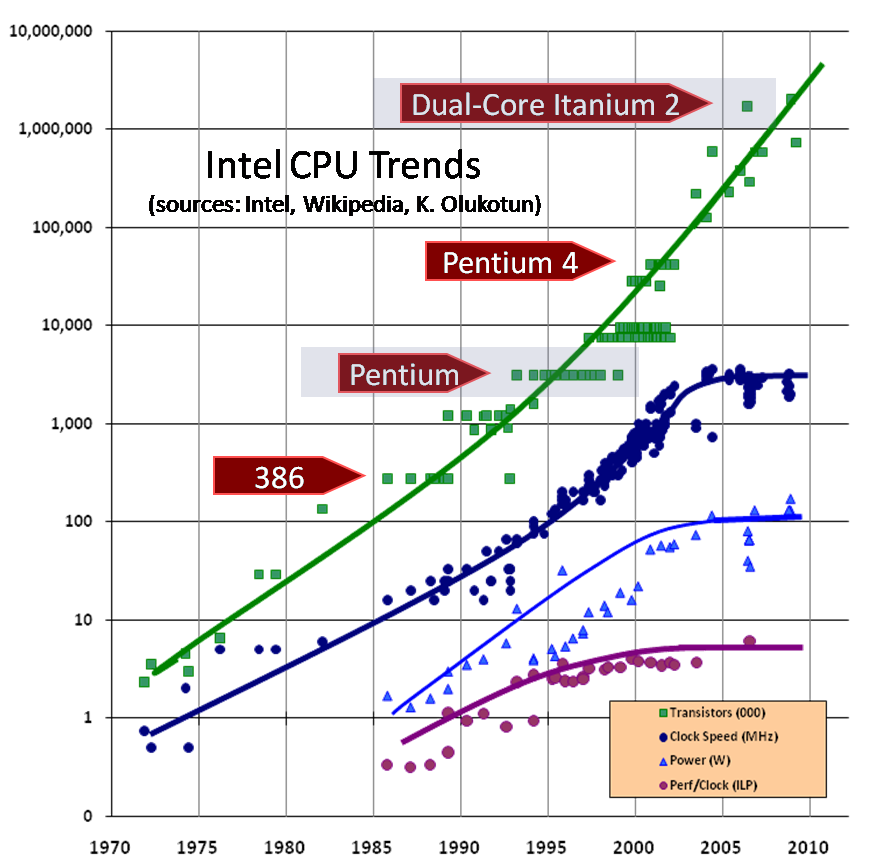
\includegraphics[width=\textwidth]{trend_graph.png}
\caption[A subset of Intel CPU introductions between 1970 and 2010]{A subset of Intel CPU introductions between 1970 and 2010. \cite{Sut05}}
\label{fig:cpu_trends}
\end{figure}

The number of transistors, shown by the green line, shows that processor performance is consistently growing at an exponential rate, which matches Moore's law. The growth of power input and clock speed are shown by the light and dark blue lines respectively. It can be seen that these values also rose exponentially, until about 2002 when they both seem to level out. This point indicates the beginning of the use of parallelism in general-purpose processors.

The problem with increasing the voltage input to the processor is that a by-product of power is heat. This was not a problem when the technique was originally applied, as cooling systems such as fans were sufficient to manage the heat output. However, as more and more power was required to increase clock speed further for each new build, the processor was giving off more and more heat until a level of heat was reached that could not be sufficiently cooled and became a danger to the computer and its environment \cite{Adv08}. This meant that processor performance matching Moore's law could not longer be attained by increasing clock speed; a new technique was required to continue growth of processing performance.

\subsection{An introduction to parallel systems}

This new technique was the use of parallelism within the processor. Operating on the principle that large problems can often be divided up into smaller, independent problems, parallel systems have more than one processing core that can each carry out an instruction on different pieces of data concurrently \cite{Got89}. With each instruction executed in parallel to another, the execution time of the instruction is 'hidden' meaning the overall runtime of the program is reduced compared to serial execution. This is the basis on which parallel systems achieve improved performance, without relying on an increase in clock speed.

Of course, this technique was not particularly new. It was used prior to 2002 for many years in the high-performance computing industry, where it was used in massively parallel supercomputers which executed large-scale calculations such as molecular dynamics and climate modelling. These machines were very specialist and not general-purpose, but their parallelism worked very well. This meant that when the time came, the technique could be taken and applied to general-purpose systems to give increased processing performance on machines that were available for use by the general public.

Most general-purpose parallel systems use a SIMD (single instruction, multiple data) architecture, another classification of processor defined in Flynn's Taxonomy \cite{Fly72}. This architecture works in a way that is best explained using a simple example of a calculation that it can perform. Imagine a $4 \times 4$ matrix of random integers, and a program that aims to find the product of these integers. A SISD architecture, which uses one core and one block of memory, would execute fifteen serial multiplications to find the product of the $4 \times 4$ matrix. However for a SIMD architecture with four cores, each with its own memory block, the $4 \times 4$ matrix can be split into four $4 \times 1$ matrices, one for each core in the processor. Parallel execution of three serial multiplications by each core can then be carried out, resulting in four partial product values which are then in turn multiplied by the master core to get the final value. Assuming each multiplication takes one clock cycle, the SISD architecture can complete the calculation in fifteen clock cycles, whereas the SIMD architecture can theoretically complete the calculation in six clock cycles. I say theoretically because parallel architectures are not as simple as serial architectures, and come with some overheads that have not yet been discussed. The main overhead associated with parallel architectures is communication between cores, which is the main focus of this paper.

\subsection{An introduction to interconnects}

Interconnects provide communication channels between cores working concurrently, and are an integral part of a parallel architecture. Let us look at the $4 \times 4$ matrix multiplication example again, this time in more detail.

The program starts off in the same way that a serial program would start, running on the master core only. Here, random integers are assigned to each position in the $4 \times 4$ matrix, arbitrarily in the case of this example. Once the matrix has been filled, the parallel section of the program can begin. The matrix is split up into rows, giving four $4 \times 1$ matrices. However for these matrices to be distributed between the four available cores, they need to be passed from the master core via an interconnect. The interconnect provides a path for data between cores, meaning the first $4 \times 1$ matrix can be passed from the master core to core[1], the second $4 \times 1$ matrix can be passed to core[2] and the third $4 \times 1$ matrix can be passed to core[3]. The fourth $4 \times 1$ matrix does not need to be passed to a different core, it remains on the master core (core[0]). Once all data has been distributed between cores, parallel processing begins as each core calculates the product of its section of the $4 \times 4$ matrix, resulting in four partial product values; one on each core. Again, interconnects are needed here to transport each partial product back to the master core, so that the final multiplication can take place. This is the end of the parallel section, and the final multiplication is done in serial resulting in the returned value of the program.

This is a very simplified example of the type of calculation parallel systems are used for, but it gives a good indication of how important interconnects are to the functionality of a SIMD architecture. However their use is not without its drawbacks, mainly the associated overheads that it adds to the system using it. For example in the program described above, extra computation is required by the system to specify a destination for each $4 \times 1$ matrix, to distribute the list of instructions to be executed by each core, and to specify the destination for each of the partial products. Another large overhead is the time taken to physically transport data across an interconnect wire. The speed of data transportation is restricted by the speed of light, roughly $3.0 \times 10^8$ m/s, and while this may seem more than sufficient for transportation rates of negligible time, let us consider the speed of modern processor clock speeds. An average clock speed in 2015 is around 2 GHz, which is equivalent to $2.0 \times 10^9$ clock cycles per second. So in one clock cycle, light travels roughly 15cm. This is not a very large distance, especially in larger scale supercomputers when interconnects may need to stretch tens or hundreds of metres. This suggests that, given the speed of modern processors, the majority of runtime in a parallel program is spent on data transfer rather than actual computation, which means that efforts to speed up the service that interconnects provide are essential for providing a further improvement of parallel processing performance.

\subsection{Interconnection networks}

An interconnection network is built up when a number of interconnects are used in a parallel architecture. In an ideal world, each core would be connected to every other core by a single interconnect, giving direct communication between all cores in a system. However in practice this is not feasible, as for every nth core added to the network, $n-1$ interconnects must also be added to maintain complete connection. This means that the number of interconnects scales by $n^2$ the number of cores, making this implementation non-scalable and not an option.

Instead, a sparsely-connected network must be used where each core is connected to a small number of other cores. As long as every core is reachable by every other core, which the network model requires, communication can then take place either directly between connected cores, or indirectly using more than one interconnect via intermediate cores. Switches can also be used in an interconnection network as intermediate nodes, which direct data down different paths in the network. These will be described in more detail later.

\subsection{Network topologies}
\label{sec:topologies}

A topology represents an abstracted layout of a network, in terms of cores/switches (nodes) and interconnects (edges). There are many different topologies that can be used, with even modern supercomputer manufacturers disagreeing about which one gives best performance \cite{Han14}. There are five main topologies: mesh, toroidal, hypercubic, tree and Clos.

\begin{figure}[H]
\centering
\subfloat[2D mesh] {
	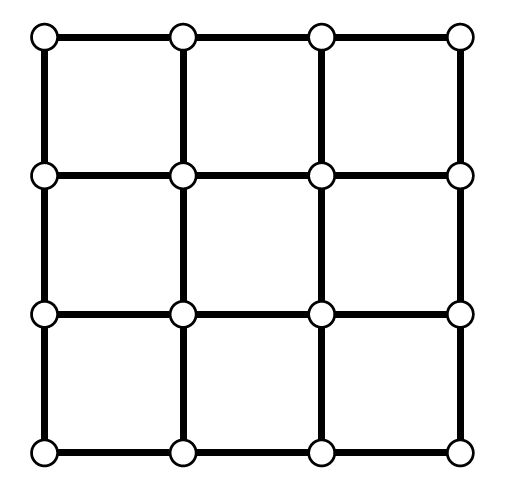
\includegraphics[width=65mm]{mesh_network.png}
}
\subfloat[2D torus] {
	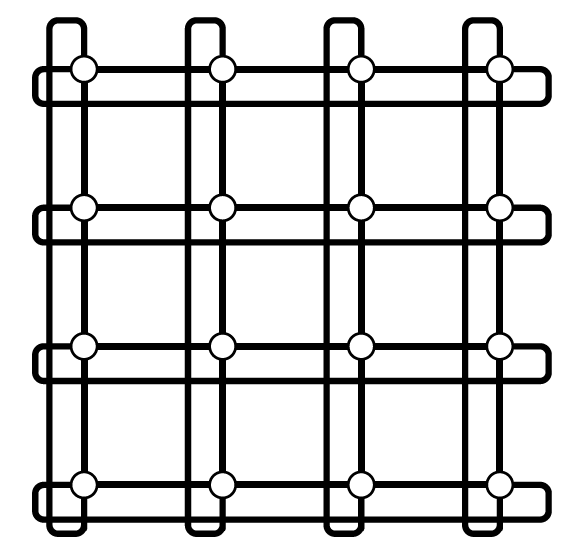
\includegraphics[width=65mm]{toroidal_network.png}
}
\newline
\subfloat[4D hypercube] {
	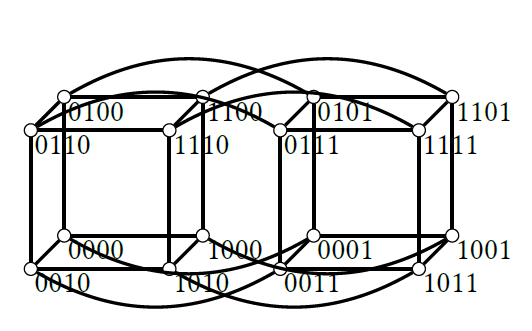
\includegraphics[width=65mm]{hypercubic_network.png}
}
\subfloat[Fat tree] {
	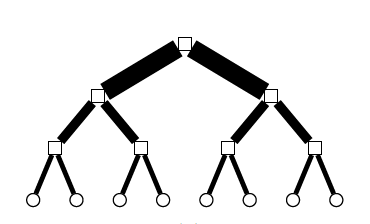
\includegraphics[width=65mm]{fat_tree_network.png}
}
\newline
\subfloat[Clos] {
	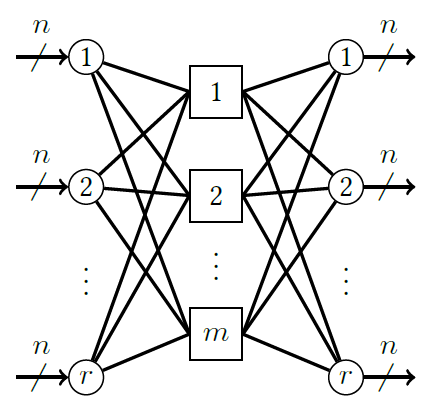
\includegraphics[width=65mm]{clos_network.png}
}
\subfloat[Bene\v{s}] {
	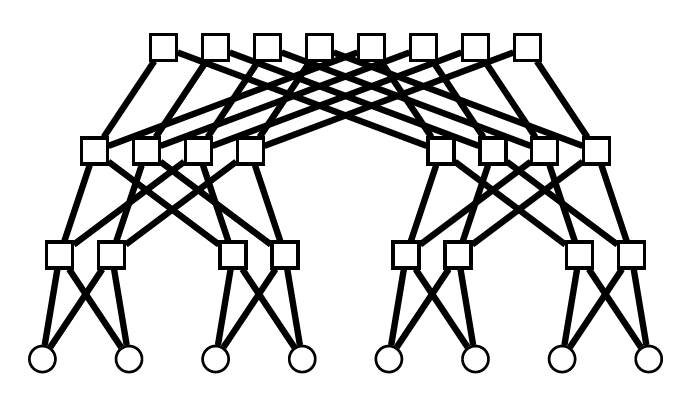
\includegraphics[width=65mm]{benes_network.png}
}
\caption[Different network topologies used in parallel architectures]{Different network topologies used in parallel architectures. \cite{Han14}}
\label{fig:topologies}
\end{figure}

Mesh and toroidal networks have a regular layout similar to arrays. Cores in mesh networks are only connected to adjacent positions in the array, with the cores in the middle of the array having more connections than the cores at the edge. Toroidal networks remove this non-uniformity, allowing cores at the edge of the array to 'wrap around' the array to connect to the adjacent node at the other end of the dimension.

Hypercubic networks have a symmetric and recursive structure. A $d+1$ dimensional hypercubic network can be constructed by connecting two d dimensional hypercubes by their matching cores. 

Tree networks have a root node connecting one or more child nodes, which in turn connect one or more child nodes until all nodes are connected. The fact that all nodes have the common root node means that every node is reachable, which is a requirement of a network topology. However because there is only one root node, traffic around this node can get quite busy when lots of communication is taking place. Fat trees address this problem, giving interconnects closer to the root of the tree more bandwidth so that more data can be transmitted on each clock cycle.

Clos networks were originally designed for use in telecommunications \cite{Clo53}. They use non-blocking switches to allow continuous transfer of data over multiple connections. Each connection has three stages: an ingress stage where data is sent from a core, a middle stage where data passes through one or more switching nodes, and an egress stage where data is received by the receiving core. The middle stage can be made up of further Clos networks, making a chain structure which gives more paths for each connecting nodes. Bene\v{s} networks are a type of Clos network, where each node is connected to exactly two other nodes \cite{Ben65}. Due to the symmetry of Clos and Bene\v{s} networks, they can be folded across the middle stage as shown in figure \ref{fig:topologies}f. This merges the ingress and egress stages by using bidirectional communications links, allowing more efficient traversal of the network.

\subsection{Routing}

A routing algorithm decides which path of a network the data is sent along during communication between two nodes. Ideally the shortest path between the two nodes is selected, however consideration of the state of the network should be taken into account to try and minimise link contention within the network. There are a number of different routing algorithms used in parallel systems, a selection of which are described below.

\subsubsection{Oblivious routing}

Oblivious routing ignores the state of the network when deciding which path should be chosen for communication. This means that it typically chooses the shortest path between two nodes, which can result in very poor use of the network in the worst case. However the worst case is an unusual scenario, and in the average case this algorithm can perform quite well with minimal overheads slowing down communication.

\subsubsection{Adaptive routing}

Adaptive routing aims to distribute communication paths across the network more evenly \cite{Dal03}. Each node uses the buffer occupancy in the nodes connected to it to choose the path with the least traffic, allowing data to be transmitted down the least congested path. However this technique is open to the risk of livelock, where the chosen path goes around in circles and the data does not progress towards its destination. This is obviously a problem, as data is not guaranteed to reach its destination in an acceptable time for efficient communication to take place.

\subsubsection{Two-phase randomised routing}

Two-phase randomised routing is another technique used to spread traffic uniformly over the network \cite{Val90}. It selects a random intermediate node somewhere in the network, and then ensures that data passes through this node on its way to its intended destination. As the name suggests, communication is split into two phases: sending the data to the intermediate node, and forwarding the data on to the destination node. Both of these phases use oblivious routing, meaning that data generally travels twice the average path length, but the addition of the random element tends to distribute traffic evenly over the network and improves communication efficiency.

\subsection{Switching}

A switching scheme handles the way in which network resources are used during communication. Switches are included in a network as intermediate nodes that forward data along a specified route to its destination node. There are a number of different switching schemes used in parallel systems, a selection of which are described below.

\subsubsection{Packet switching}

Packet switching is a very commonly used switching scheme. It splits the piece of data to be transmitted up into fixed length parts called packets, and then each of these packets is transmitted independently of one another to their destination. Once all the packets have reached their destination, the data is then reassembled and reconstructed ready for use by the node. The fact that packets are send independently means that in some situations they can be sent concurrently down different paths of the network, improving communication efficiency.

\subsubsection{Circuit switching}

Circuit switching reserves a complete path from source node to destination node across the network before communication has begun, meaning that the links in the reserved path cannot be used by any other communication before the initial communication is complete. This technique reduces the number of decisions made during communication regarding the state of the network, however restricting certain links in the network from being used can result in a waste of available bandwidth, making communication sometimes inefficient.

\subsubsection{Wormhole switching}

Wormhole switching is a similar technique to packet switching, but goes a step further by dividing up packets again before transmission. Each packet is split up into a sequence of flits, which are then transmitted in the same manner as packet switching. However due to the smaller size of each flit, each packet is pipelined in the network reducing latency and buffer requirement. This can important in general-purpose systems where buffer size can be chosen independently of potentially differing packet sizes.

\subsection{Flow control}

Flow control algorithms deal with the allocation of network resources, such as buffer space and bandwidth used by each data packet \cite{Jon97}. This allows the network to avoid buffer overflow, and increases the efficiency of communication. There are two main flow control schemes: credit-based flow control, and virtual channel flow control.

\subsubsection{Credit-based control flow}

During communication, credit-based control flow only allows transmission on a link if there is sufficient buffer space in the next node on the route. Each node has a counter of available buffer space on its input, and if the count value indicates that the next packet would cause a buffer flow, transmission is blocked. When there is a lot of traffic on the network, this technique can cause a backup of traffic where there are no suitable routes for a packet to be sent down, so the packet must wait until more buffer space in the next node becomes available. In very heavy traffic, this can halt communication altogether as no more packets can be injected into the network.

\subsubsection{Virtual channel control flow}

Virtual channels can be implemented in a network to avoid the problem of potential blockages which halt data transmission across a certain link \cite{Dal92}. A virtual channel consists of a buffer and associated state information, and multiple virtual channels can be allocated to a single link in the network \cite{Dal87}. The virtual channels provide multiple buffer spaces for packets coming into the node, and when data in a channel is ready to progress, it can be assigned access to the physical link and communication can be continued. The addition of virtual channels to a link is analogous to adding new lanes to a motorway; if a car breaks down on one of the lanes, traffic can still pass on the other available lanes. In the same way, if data stored in the buffer of one of the virtual channels is unable to progress through the network for a certain reason, the other virtual channels can be used by data packets which are able to progress.

\subsection{Modern interconnection networks}

The final part of this section looks at two examples of modern interconnection networks used in general-purpose parallel systems. The two examples in question are InfiniBand and the IBM Blue Gene/L 3D torus network.

\subsubsection{InfiniBand}

InfiniBand is an industry-wide networking standard developed in 2000 by a consortium of companies belonging to the InfiniBand Trade Association \cite{Hen11}. It is used predominantly in massively parallel supercomputers, where its flexibility regarding network topology and use of routing algorithms are popular with manufacturing companies which like to have control over the schemes used in their products. InfiniBand uses a switch-based interconnect that supports data transmission speeds of 2 to 120 Gbp/link, where each link can reach a length of up to 300m. It uses cut-through switching, a variation of packet switching, 16 virtual channels per link, and credit-based control flow. This allows data of up to 512KB to be transmitted between cores as a single message, however approximately 90\% of messages are less than 512 bytes meaning the maximum message length is rarely transmitted. 

\subsubsection{IBM Blue Gene/L 3D Torus Network}

In 2005, the IBM Blue Gene/L was the largest, most powerful supercomputer in the world, according to www.top500.org \cite{Hen11}. It used a 32x32x64 3D torus interconnection network, which connected all of its 64000 nodes. When communication between two nodes was required, either node could be used for  communication protocol processing while the other may have been carrying out other computation. Packet sizes ranged from 32 bytes to 256 bytes, with an 8 byte header containing routing, virtual channel and link-level flow control, as well as a 1 byte CRC for packet validation. Virtual cut-through switching and credit-based control flow were again used, along with various other schemes which provided the low latency and high bandwidth requirements of a machine designed to execute computation as quickly and efficiently as possible.


\newpage
\section{Specification}



\newpage
\section{Design}



\newpage
\section{Implementation}



\newpage
\section{Testing}



\newpage
\section{Results}



\newpage
\section{Conclusion}



\newpage
\section{References}

\begin{thebibliography}{30}

\bibitem[Adv08]{Adv08} Adve, S. V. et al. (November 2008). \textit{'Parallel Computing Research at Illinois: The UPCRC Agenda'}. Parallel@Illinois, University of Illinois at Urbana-Champaign.

\bibitem[Ben65]{Ben65} Bene\v{s}, V. E. (1965). \textit{Mathematical Theory of Connecting Networks and Telephone Traffic}. Mathematics in Science and Engineering. Academic Press.

\bibitem[Clo53]{Clo53} Clos, C. (March 1953). \textit{'A study of non-blocking switching networks'}. Bell System Technical Journal 32 (2): 406-424. doi:10.1002/j.1538-7305.1953.tb01433.x.

\bibitem[Dal87]{Dal87} Dally, W. J., Seitz, C. L. (May 1987). \textit{Deadlock-free message routing in multiprocessor interconnection networks}. Computers, IEEE Transactions on, 100 (5): 547-553.

\bibitem[Dal92]{Dal92} Dally, W. J. (March 1992). \textit{Virtual-channel flow control}. IEEE Transactions on Parallel and Distributed Systems, 3 (2): 194-205.

\bibitem[Dal03]{Dal03} Dally, W. J., Towles, B. (2003). \textit{Principles and Practices of Interconnection Networks}. Morgan Kaufmann.

\bibitem[Fly72]{Fly72} Flynn, M. J. (September 1972). \textit{'Some Computer Organizations and Their Effectiveness'}. IEEE Trans. Comput. C-21 (9): 948-960. doi:10.1109/TC.1972.5009071.

\bibitem[Got89]{Got89} Gottlieb, A. Almasi, G. (1989). \textit{Highly parallel computing}. Redwood City, Calif.: Benjamin/Cummings. ISBN 0-8053-0177-1.

\bibitem[Han14]{Han14} Hanlon, J. W. (March 2014). \textit{Scalable abstractions for general-purpose parallel computation}. p. 44-48, 62.

\bibitem[Hen11]{Hen11} Hennessy, J. L., Patterson, D. A. (2011). \textit{Computer Architecture: A Quantitative Approach}. Online appendix F, retrieved from http://booksite.elsevier.com/9780123838728/references.php

\bibitem[Iba08]{Iba08} Ibaroudene, Djaffer. (Spring 2008). \textit{'Parallel Processing, EG6370G: Chapter 1, Motivation and History'}. St. Mary's University, San Antonio, TX.

\bibitem[Jon97]{Jon97} Jones, A. M. et al. (1997). \textit{The Network Designer's Handbook}. IOS Press, 1st edition.

\bibitem[Lam04]{Lam04} Lammle, T. (2004). \textit{CCNA Study Guide} (Fourth edition). Sybex Inc. ISBN 0-7821-4311-3.

\bibitem[Moo65]{Moo65} Moore, G. E. (1965). \textit{'Cramming more components onto integrated circuits'}. Electronics Magazine. p. 4.

\bibitem[Sut05]{Sut05} Sutter, H. (March 2005). \textit{'The free lunch is over'}. Dr Dobb's Journal, 30(3). Online version, updated August 2009.

\bibitem[Toy86]{Toy86} Toy, W., Zee, B. (1986). \textit{Computer Hardware/Software Architecture}. Prentice Hall. ISBN 0-13-163502-6.

\bibitem[Val90]{Val90} Valiant, L. G. (1990). \textit{General purpose parallel architectures}. In Handbook of theoretical computer science (vol. A): algorithms and complexity, p. 943-973. MIT Press.

\end{thebibliography}


\end{document}